 \documentclass{beamer}
\mode<presentation>
\usepackage{amsmath}
\usepackage{amssymb}
%\usepackage{advdate}
\usepackage{graphicx}
\usepackage{adjustbox}
\usepackage{subcaption}
\usepackage{enumitem}
\usepackage{multicol}
\usepackage{mathtools}
\usepackage{listings}
\usepackage{url}
\def\UrlBreaks{\do\/\do-}
\usetheme{Boadilla}
\usecolortheme{lily}
\let\vec\mathbf
\setbeamertemplate{footline}
{
  \leavevmode%
  \hbox{%
  \begin{beamercolorbox}[wd=\paperwidth,ht=2.25ex,dp=1ex,right]{author in head/foot}%
    \insertframenumber{} / \inserttotalframenumber\hspace*{2ex} 
  \end{beamercolorbox}}%
  \vskip0pt%
}
\setbeamertemplate{navigation symbols}{}

\providecommand{\nCr}[2]{\,^{#1}C_{#2}} % nCr
\providecommand{\nPr}[2]{\,^{#1}P_{#2}} % nPr
\providecommand{\mbf}{\mathbf}
\providecommand{\pr}[1]{\ensuremath{\Pr\left(#1\right)}}
\providecommand{\qfunc}[1]{\ensuremath{Q\left(#1\right)}}
\providecommand{\sbrak}[1]{\ensuremath{{}\left[#1\right]}}
\providecommand{\lsbrak}[1]{\ensuremath{{}\left[#1\right.}}
\providecommand{\rsbrak}[1]{\ensuremath{{}\left.#1\right]}}
\providecommand{\brak}[1]{\ensuremath{\left(#1\right)}}
\providecommand{\lbrak}[1]{\ensuremath{\left(#1\right.}}
\providecommand{\rbrak}[1]{\ensuremath{\left.#1\right)}}
\providecommand{\cbrak}[1]{\ensuremath{\left\{#1\right\}}}
\providecommand{\lcbrak}[1]{\ensuremath{\left\{#1\right.}}
\providecommand{\rcbrak}[1]{\ensuremath{\left.#1\right\}}}
\theoremstyle{remark}
\newtheorem{rem}{Remark}
\newcommand{\sgn}{\mathop{\mathrm{sgn}}}
\providecommand{\abs}[1]{\vert#1\vert}
\providecommand{\res}[1]{\Res\displaylimits_{#1}} 
\providecommand{\norm}[1]{\lVert#1\rVert}
\providecommand{\mtx}[1]{\mathbf{#1}}
\providecommand{\mean}[1]{E[ #1 ]}
\providecommand{\fourier}{\overset{\mathcal{F}}{ \rightleftharpoons}}
%\providecommand{\hilbert}{\overset{\mathcal{H}}{ \rightleftharpoons}}
\providecommand{\system}[1]{\overset{\mathcal{#1}}{ \longleftrightarrow}}
%\providecommand{\system}{\overset{\mathcal{H}}{ \longleftrightarrow}}
	%\newcommand{\solution}[2]{\vec{Solution:}{#1}}
%\newcommand{\solution}{\noindent \vec{Solution: }}
\providecommand{\dec}[2]{\ensuremath{\overset{#1}{\underset{#2}{\gtrless}}}}
\newcommand{\myvec}[1]{\ensuremath{\begin{pmatrix}#1\end{pmatrix}}}


\lstset{
%language=C,
frame=single, 
breaklines=true,
columns=fullflexible
}
\lstset{
  language=C,
  basicstyle=\ttfamily\footnotesize,
  keywordstyle=\color{blue}\bfseries,
  commentstyle=\color{gray}\itshape,
  stringstyle=\color{orange},
  numbers=left,
  numberstyle=\tiny\color{gray},
  breaklines=true,
  frame=single,
  showstringspaces=false,
  tabsize=4,
  captionpos=b
}
\numberwithin{equation}{section}
\lstset{
  language=Python,
  basicstyle=\ttfamily\small,
  keywordstyle=\color{blue},
  stringstyle=\color{orange},
  numbers=left,
  numberstyle=\tiny\color{gray},
  breaklines=true,
  showstringspaces=false
}

\title{Problem 3.4.4}
\author{Sujal Rajani}

\date{\today} 
\begin{document}

\begin{frame}
\titlepage
\end{frame}

\section{Question}
\begin{frame}{Question}
\textbf{Question}:
\noindent Construct a rectangle whose adjacent sides are of lengths 5cm and 3.5cm.
\end{frame}
\begin{frame}{Solution}
\textbf{SOLUTION}
 as  mentioned in question adjacent sides are of lengths 5cm and 3.5cm.
 \\
as nothing is mentioned in question about the points :
\\
so we are taking rectangle as ABCD :
\\
 where position vector of respective points are :
 \\
 \begin{align*}
     \vec{A}=\myvec{0\\0}, \vec{B}=\myvec{0\\5}, \vec{C}=\myvec{3\\5},\vec{D}=\myvec{3\\0},
 \end{align*}
 \end{frame}
\begin{frame}{Solution}
 our assumed coordinates are satisfying all the properties of rectangle :
 \begin{align*}
     (\vec{B}-\vec{A})^\top(\vec{C}-\vec{B})=0
     \\
      (\vec{C}-\vec{B})^\top(\vec{D}-\vec{C})=0
      \\
       (\vec{D}-\vec{C})^\top(\vec{A}-\vec{D})=0
        \\
        (\vec{A}-\vec{D})^\top(\vec{B}-\vec{A})=0
 \end{align*}
 \begin{align*}
     (\vec{B}-\vec{A})^\top(\vec{B}-\vec{A})=25
     \\
     (\vec{C}-\vec{B})^\top(\vec{C}-\vec{B})=9
     \\
      (\vec{D}-\vec{C})^\top (\vec{D}-\vec{C})=25
      \\
      (\vec{A}-\vec{D})^\top(\vec{A}-\vec{D})=9
 \end{align*}
     \end{frame}
       \begin{frame}[fragile]
    \begin{figure}[H]
    \centering
    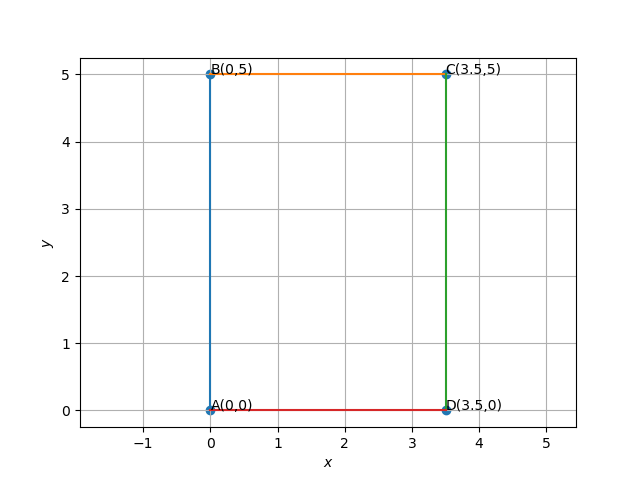
\includegraphics[width = 0.6\columnwidth]{../figs/img.png}
    \caption*{}
    \label{figs}
\end{figure}
\end{frame}
\section{ C Code}
\begin{frame}[fragile]
\frametitle{C Code }
\begin{lstlisting}[language=C]
#include <stdio.h>

int main() {
    // Rectangle vertices
    int Ax = 0, Ay = 0;
    int Bx = 0, By = 5;
    int Cx = 3, Cy = 5;
    int Dx = 3, Dy = 0;

 

\end{lstlisting}
\end{frame}

\begin{frame}[fragile]
\frametitle{C Code }
\begin{lstlisting}[language=C]
       printf("Coordinates of the rectangle are:\n");
    printf("A(%d, %d)\n", Ax, Ay);
    printf("B(%d, %d)\n", Bx, By);
    printf("C(%d, %d)\n", Cx, Cy);
    printf("D(%d, %d)\n", Dx, Dy);

    return 0;
}
\end{lstlisting}
\end{frame}



\begin{frame}[fragile]
\frametitle{Python Code for Plotting}
\begin{lstlisting}[language=Python]
import numpy as np
import matplotlib.pyplot as plt
from line.funcs import *
# from triangle.funcs import *
# from conics.funcs import circ_gen
# if using termux
import subprocess
import shlex
# end if

\end{lstlisting}

\end{frame}
\section{Python Code}
\begin{frame}[fragile]
\frametitle{Python Code for Plotting}
\begin{lstlisting}[language=Python]

\end{lstlisting}

\end{frame}
\begin{frame}[fragile]
\frametitle{Python Code for Plotting}
\begin{lstlisting}[language=Python]
# Rectangle vertices
A = np.array([0,0]).reshape(-1,1)
B = np.array([0,5]).reshape(-1,1)
C = np.array([3,5]).reshape(-1,1)
D = np.array([3,0]).reshape(-1,1)

coords = np.block([[A,B,C,D]])
# Generate only rectangle sides
AB = line_gen(A,B)
BC = line_gen(B,C)
CD = line_gen(C,D)
DA = line_gen(D,A)
\end{lstlisting}

\end{frame}
\begin{frame}[fragile]
\frametitle{Python Code for Plotting}
\begin{lstlisting}[language=Python]


# Plot sides
plt.plot(AB[0,:],AB[1,:], label='AB')
plt.plot(BC[0,:],BC[1,:], label='BC')
plt.plot(CD[0,:],CD[1,:], label='CD')
plt.plot(DA[0,:],DA[1,:], label='DA')
# Scatter points
plt.scatter(coords[0,:],coords[1,:])
plt.text(A[0],A[1],"A(0,0)") 
plt.text(B[0],B[1],"B(0,5)")
plt.text(C[0],C[1],"C(3,5)")
plt.text(D[0],D[1],"D(3,0)")

\end{lstlisting}

\end{frame}
\begin{frame}[fragile]
\frametitle{Python Code for Plotting}
\begin{lstlisting}[language=Python]
plt.xlabel('$x$')
plt.ylabel('$y$')
plt.legend(loc='best')
plt.grid(True)
plt.axis('equal')

plt.savefig('../figs/img.png')
plt.show()
\end{lstlisting}

\end{frame}
\end{document}